\documentclass{article}
\usepackage[a4paper, margin=2.5cm, headheight=13pt]{geometry}
\usepackage[french]{babel}
\usepackage{fancyhdr}
\usepackage{tikz}
\usepackage{xcolor}
\usetikzlibrary{positioning, calc}
\usepackage{graphicx}

%define_color
\definecolor{bleu}{rgb}{0,0.52,1}
\definecolor{vert}{rgb}{0.45,0.82,0}

% Subfigures
\usepackage{caption}
\usepackage{subcaption}

% Définir la pagination etc.
\pagestyle{fancy}
\fancyhf{}
\lhead{MICRO-315 Miniprojet} 
\rhead{Les aventures de Jean-Bot}
\fancyfoot
{
    \begin{tikzpicture}[remember picture,overlay]
            \node[] (chat) at ($(current page.south)+(0,1.5)$) {
\includegraphics[width=1cm]{images/amour.pdf}};
            \node[] () at ($(chat)+(0,0.04)$) {\thepage};
            \node[] () at ($(chat)-(1,0)$) {
\includegraphics[width=1cm]{images/kawwai.pdf}};
            \node[] () at ($(chat)+(1,0)$) {\scalebox{-1}[1]{
\includegraphics[width=1cm]{images/kawwai.pdf}}};
    \end{tikzpicture}
}

\begin{document}
    \begin{titlepage}
        \vspace*{\fill}
        \begin{center}
            \begin{tikzpicture}[remember picture, overlay]
                \node[] at (current page.center) {\includegraphics[angle=90, width=\paperwidth]{images/background.jpg}};
                \fill[color = white, opacity = 0.9, rounded corners = 2ex] (-10,5) rectangle (10,-5);
                \node (titre) at (0,0)
                    {
                        \begin{tabular}{c}
                            \hline
                            \\
                            \huge\it Les aventures incroyables de \\
                            \\
                            \Huge\bf Jean-Bot Baptiste I\\
                            \\
                            \huge\it Le raccourceur des circuits\\
                            \\
                            \hline
                        \end{tabular}
                    };
                \node[left]  at (titre.west) {
\includegraphics[width=5cm]{images/kawwai.pdf}};
                \node[right] at (titre.east) {\scalebox{-1}[1]{
\includegraphics[width=5cm]{images/kawwai.pdf}}};
                \node[above] at (titre.north) {\textbf{\large MICRO-315 Miniprojet}};
                \node[below] at (titre.south) {\textit{\large Un projet de robotique de Julian Donevsky et Olof Lissmats}};
            \end{tikzpicture}
        \end{center}
        \vspace{5cm}
        \vspace*{\fill}
    \end{titlepage}

    \thispagestyle{empty}

    \tableofcontents

    \newpage

    \setcounter{page}{1}

    \section{Introduction}

    Dans le cadre de ce projet, nous avons créé un programme qui permet au robot de danser sur une musique en particulier en fonction d'un drapeau de pays que l'utilisateur lui présente.
    Le robot utilise ses capteurs de proximités infrarouges pour s'assurer qu'aucun obstacle ne bloque son chemin lorsqu'il danse. 
    Si c'est le cas, il arrête temporairement sa danse jusqu'à ce que l'obstacle soit dégagé.

    \section{Métholodogie}
    
    \subsection{Schéma général du programme}
    \begin{figure}[!ht]
        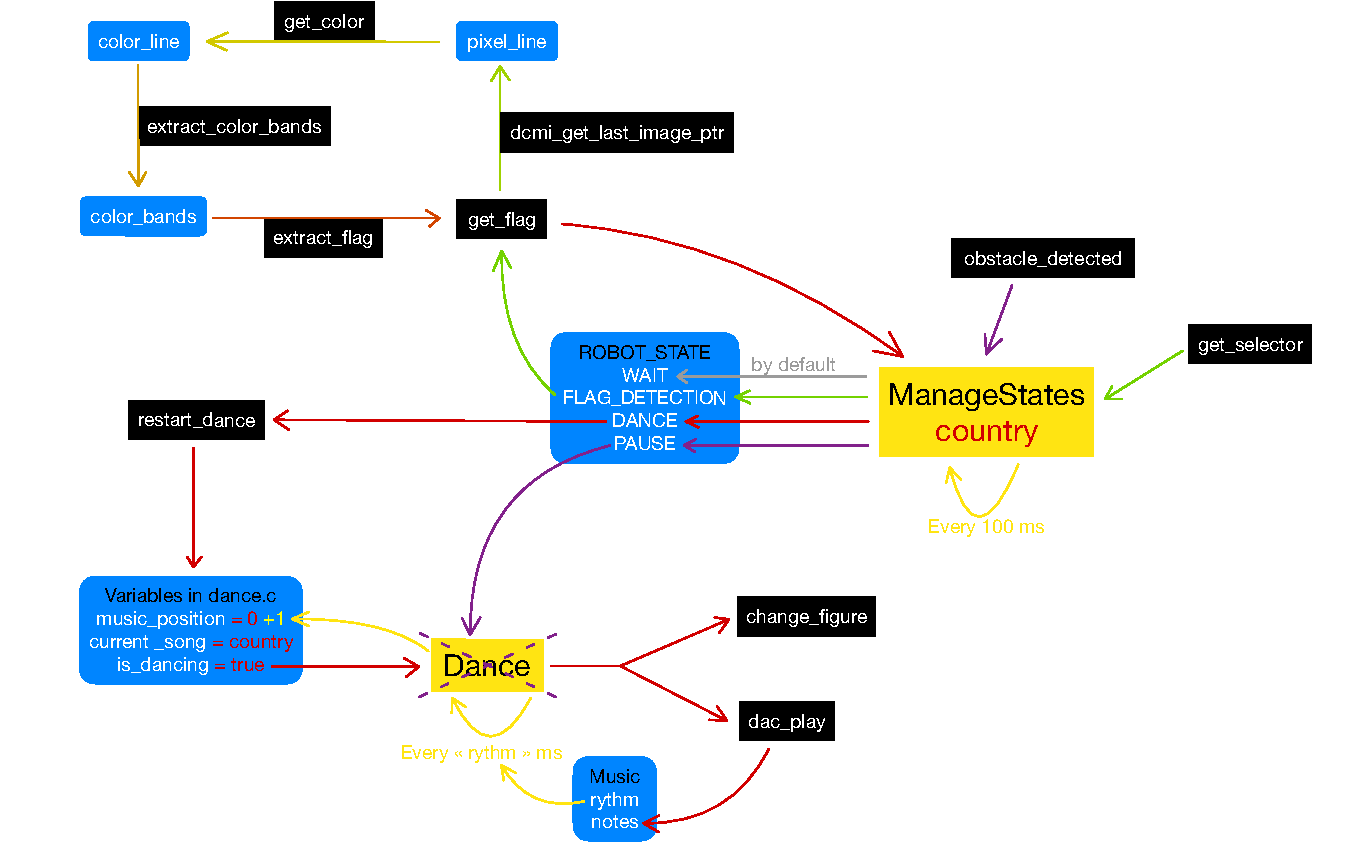
\includegraphics[scale=0.75]{images/code-structure.pdf}
        \caption{Schéma général du programme. En jaune les threads, en noir les fonctions et en bleu (rouge dans le cas de country) les variables utiles au bon déroulement du programme.}
        \label{fig:structure} % Pour référer à cette figure dans le texte
    \end{figure}

    L'utilisateur tourne le selecteur (peu importe de combien de cran). 
    La détection se fait en appellant la fonction \textbf{get$\_$selector} dans le thread \colorbox{yellow}{\textbf{ManagesStates}}, qui met ensuite l'état du robot à \textcolor{bleu}{FLAG$\_$DETECTION} ce qui a pour conséquence d'appeler la fonction \textbf{get$\_$flag} (\textcolor{vert}{flèche en vert}). \\ \par
    
    A chaque appel de \textbf{get$\_$flag}, une image sur la caméra est capturée et une ligne de pixel est stockée dans la variable \textcolor{bleu}{pixel$\_$line}. 
    Chaque pixel de \textcolor{bleu}{pixel$\_$line} est ensuite convertit en une couleur (blanc, rouge, vert, bleu, indéfini) grâce à la fonction \textbf{get$\_$color}, puis stocké dans \textcolor{bleu}{color$\_$line}. 
    La fonction \textbf{extract$\_$color$\_$bands} s'occupe d'analyser \textcolor{bleu}{color$\_$line} (voir section \ref{extract_color_bands}) pour en extraire les grandes bandes de même couleur correspondant au drapeau présenté. 
    Finalement, \textbf{extract$\_$flag} en déduit le drapeau et le retourne à \textbf{get$\_$flag}. 
    Si la fonction \textbf{get$\_$flag} n'a pas réussi à trouver le drapeau, elle continue de s'exécuter en boucle jusqu'à obtenir un drapeau connu pendant au maximum 10 secondes. 
    Passé ce délai, le robot retourne dans l'état \textcolor{bleu}{WAIT}. \\ \par
    
    Lorsqu'un drapeau connu est enfin trouvé, le thread \colorbox{yellow}{\textbf{ManagesStates}} appelle la fonction \textbf{restart$\_$dance} qui réveille le thread \colorbox{yellow}{\textbf{Dance}} (\textcolor{red}{flèche en rouge}). 
    En effet, la variable \textcolor{bleu}{is$\_$dancing} est initialisée à \textit{false} et inhibe le thread en le faisant simplement dormir dans une boucle de 100 ms. 
    Lorsqu'elle passe à \textit{true}, celui-ci sort de son sommeil et commence à jouer la musique \textcolor{bleu}{current$\_$song} (changée à la musique du pays détecté par \textbf{restart$\_$dance} grâce à une look up table). 
    A chaque note jouée, les fonctions \textbf{change$\_$figure} et \textbf{dac$\_$play} sont appelée pour changer de mouvement de dance en activant de façon aléatoire les moteurs et jouer le son voulu, respectivement. 
    De plus, la variable \textcolor{bleu}{music$\_$position} indiquant quelle note et rythme jouer de la structure \textcolor{bleu}{Music} est incrémentée. \\ \par
    
    A chaque appel de \colorbox{yellow}{\textbf{ManagesStates}}, \textbf{obstacle$\_$detected} est appelé pour vérifier qu'aucun obstacle n'obstrue le chemin du robot lorsqu'il danse. Si tel est le cas, le robot passe en mode \textcolor{bleu}{PAUSE}, ce qui a pour conséquence d'inhiber le thread \colorbox{yellow}{\textbf{Dance}} en le faisant retourner dans sa boucle de sommeil de 100 ms. Une fois l'obstacle enlevé, le robot continue sa danse en reprenant là où il s'était arrêté. Notons que l'état \textcolor{bleu}{PAUSE} n'affecte nullement la détection de drapeau puisqu'une fois que le robot est dans l'état \textcolor{bleu}{FLAG$\_$DETECTION}, il ne peut pas en sortir pendant 10 secondes, à moins de détecter un drapeau.

    \subsection{La fonction extract$\_$color$\_$bands}
    \label{extract_color_bands}
    \begin{figure}[!ht]
        \centering
        \begin{subfigure}{\textwidth}
            \begin{center}
                \begin{tikzpicture}[scale=0.3]
                    \foreach \i in {1,...,4}
                    {
                        \draw[fill=gray] (\i,0) rectangle (\i+1,2);
                    }
                    \foreach \i in {5,...,8}
                    {
                        \draw[fill=red] (\i,0) rectangle (\i+1,2);
                    }
                    \foreach \i in {9,...,11}
                    {
                        \draw[fill=green] (\i,0) rectangle (\i+1,2);
                    }
                    \foreach \i in {12,...,13}
                    {
                        \draw (\i,0) rectangle (\i+1,2);
                    }
                    \foreach \i in {14,...,23}
                    {
                        \draw[fill=blue] (\i,0) rectangle (\i+1,2);
                    }
                    \foreach \i in {24,...,27}
                    {
                        \draw (\i,0) rectangle (\i+1,2);
                    }
                    \draw[fill=green] (28,0) rectangle (29,2);
                    \foreach \i in {29,...,34}
                    {
                        \draw (\i,0) rectangle (\i+1,2);
                    }
                    \foreach \i in {35,...,44}
                    {
                        \draw[fill=red] (\i,0) rectangle (\i+1,2);
                    }
                \end{tikzpicture}
            \end{center}
            \caption{Une fois les valeurs RGB de chaque pixel sont convertits à des couleurs, elles sont stockées de cette manière. La couleur grise représente une couleur non définie. La caméra fournit en fait une ligne de 640 pixels, mais dans cet exemple seulement 40 sont représentés.}
        \end{subfigure}

        \vspace{5mm}

        \begin{subfigure}{\textwidth}
            \begin{center}
                \begin{tikzpicture}[scale=0.4]
                    \draw[fill=gray]  (0,3) rectangle (1,5) node[midway] (A) {};
                    \draw[fill=red]   (1,3) rectangle (2,5);
                    \draw[fill=green] (2,3) rectangle (3,5);
                    \draw[fill=white] (3,3) rectangle (4,5);
                    \draw[fill=blue]  (4,3) rectangle (5,5);
                    \draw[fill=white] (5,3) rectangle (6,5);
                    \draw[fill=green] (6,3) rectangle (7,5);
                    \draw[fill=white] (7,3) rectangle (8,5);
                    \draw[fill=red]   (8,3) rectangle (9,5);
                    \node[anchor=east] () at ($(A)-(1,0)$) {\texttt{color\_groups:}};

                    \draw (0,0) rectangle (1,2) node[midway] (B) {\texttt{4}};
                    \draw (1,0) rectangle (2,2) node[midway] {\texttt{4}};
                    \draw (2,0) rectangle (3,2) node[midway] {\texttt{3}};
                    \draw (3,0) rectangle (4,2) node[midway] {\texttt{2}};
                    \draw (4,0) rectangle (5,2) node[midway] {\texttt{10}};
                    \draw (5,0) rectangle (6,2) node[midway] {\texttt{4}};
                    \draw (6,0) rectangle (7,2) node[midway] {\texttt{1}};
                    \draw (7,0) rectangle (8,2) node[midway] {\texttt{6}};
                    \draw (8,0) rectangle (9,2) node[midway] {\texttt{10}};
                    \node[anchor=east] () at ($(B)-(1,0)$) {\texttt{size\_of\_groups:}};
                \end{tikzpicture}
            \end{center}
            \caption{Les pixels sont groupés en fonction de leurs couleurs dans les deux arrays \texttt{color\_groups} et \texttt{size\_of\_groups} qui contiennent la couleur et la taille des groupes respectivement.}
        \end{subfigure}

        \vspace{5mm}

        \begin{subfigure}{\textwidth}
            \begin{center}
                \begin{tikzpicture}[scale=0.4]
                    \draw[fill=gray]  (0,3) rectangle (1,5) node[midway] (A) {};
                    \draw[fill=red]   (1,3) rectangle (2,5);
                    \draw[fill=blue]  (2,3) rectangle (3,5);
                    \draw[fill=white] (3,3) rectangle (4,5);
                    \draw[fill=white] (4,3) rectangle (5,5);
                    \draw[fill=red]   (5,3) rectangle (6,5);
                    \draw[fill=gray]  (6,3) rectangle (7,5);
                    \node[anchor=east] () at ($(A)-(1,0)$) {\texttt{color\_groups:}};

                    \draw (0,0) rectangle (1,2) node[midway] (B) {\texttt{4}};
                    \draw (1,0) rectangle (2,2) node[midway] {\texttt{4}};
                    \draw (2,0) rectangle (3,2) node[midway] {\texttt{10}};
                    \draw (3,0) rectangle (4,2) node[midway] {\texttt{4}};
                    \draw (4,0) rectangle (5,2) node[midway] {\texttt{6}};
                    \draw (5,0) rectangle (6,2) node[midway] {\texttt{10}};
                    \draw (6,0) rectangle (7,2) node[midway] {\texttt{?}};
                    \node[anchor=east] () at ($(B)-(1,0)$) {\texttt{size\_of\_groups:}};
                \end{tikzpicture}
            \end{center}

            \caption{Les groupes avec une taille supérieur à une seuile spécifique, ici 3, sont placés au début des arrays, c'est à dire que les groupes trop petits sont supprimés. Cela se fait pour ammortir l'effet de bruit.}
        \end{subfigure}

        \vspace{5mm}

        \begin{subfigure}{\textwidth}
            \begin{center}
                \begin{tikzpicture}[scale=0.4]
                    \draw[fill=gray]  (0,3) rectangle (1,5) node[midway] (A) {};
                    \draw[fill=red]   (1,3) rectangle (2,5);
                    \draw[fill=blue]  (2,3) rectangle (3,5);
                    \draw[fill=white] (3,3) rectangle (4,5);
                    \draw[fill=red]   (4,3) rectangle (5,5);
                    \draw[fill=gray]  (5,3) rectangle (6,5);
                    \node[anchor=east] () at ($(A)-(1,0)$) {\texttt{color\_groups:}};

                    \draw (0,0) rectangle (1,2) node[midway] (B) {\texttt{4}};
                    \draw (1,0) rectangle (2,2) node[midway] {\texttt{4}};
                    \draw (2,0) rectangle (3,2) node[midway] {\texttt{10}};
                    \draw (3,0) rectangle (4,2) node[midway] {\texttt{10}};
                    \draw (4,0) rectangle (5,2) node[midway] {\texttt{10}};
                    \draw (5,0) rectangle (6,2) node[midway] {\texttt{?}};
                    \node[anchor=east] () at ($(B)-(1,0)$) {\texttt{size\_of\_groups:}};
                \end{tikzpicture}
            \end{center}

            \caption{Les groupes consécutives ayant la même couleur sont fusionnés, et les groupes suivants sont décalés d'un placement.}
        \end{subfigure}

        \vspace{5mm}

        \begin{subfigure}{\textwidth}
            \begin{center}
                \begin{tikzpicture}[scale=0.4]
                    \draw[fill=gray]  (0,3) rectangle (1,5) node[midway] (A) {};
                    \draw[fill=blue]  (1,3) rectangle (2,5);
                    \draw[fill=white] (2,3) rectangle (3,5);
                    \draw[fill=red]   (3,3) rectangle (4,5);
                    \draw[fill=gray]  (4,3) rectangle (5,5);
                    \node[anchor=east] () at ($(A)-(1,0)$) {\texttt{color\_groups:}};
                \end{tikzpicture}
            \end{center}

            \caption{Les groupes d'une taille inférieure d'une seuile spécifique, ici 8, sont fusionnés avec les groupes non-définis entourants.}
        \end{subfigure}
        \caption{Un schéma qui explique comment fonctionne la détection des drapeaux.}
    \end{figure}

    \section{Problèmes apparus lors du projet}


    \section{Points à améliorer}
    Il y a maintes points à améliorer afin d'augmenter la qualité du robot, dont les plus importants sont présentés ci-dessous.

    \subsection{Créer un thread propre pour la détection d'obstacles}
    Dans l'état actuel des choses le robot vérifie l'absence d'obstacles en appellant une fonction au début du thread qui gère les inputs et les états.
    Par conséquent, un obstacle peut se présenter après cet appel, lorsque le robot est occupé par d'autres tâches, sans causer un arrêt d'activité.
    Cela se produit par exemple pendant la détection des drapeaux où le robot est bloqué dans une boucle.

    L'ajout d'une thread comlètement dédiée à la détection d'obstacle permettrait d'y réagir à chaque instant.
    En revanche cela impliquerait aussi une nécessité de faire communiquer cette thread avec les autres, c'est à dire introduire plus de variables globales.
    La raison pour laquelle cela n'est pas encore fait est une manque de temps et la reorganisation du code nécessaire.

    \subsection{Rendre la détection de couleurs plus fiable}
    La caméra du robot fournit une image de 640 fois 480 pixels sous le format RGB565.
    Cela signifie que l'intensité de rouge, vert et bleu sont représentés sur 5, 6 et 5 pixels respectivement.
    Afin de déterminer la couleur représentée, les écarts entre ces trois valeurs sont analysées.
    Si R dépasse G et B par un seuil spécifique, c'est admis que c'est bien rouge qui est représenté.
    La détection de vert et bleu se fait de la même façon, et au cas de blanc, le test et fort ressemblant.
    
    Le problème de cette démarche est que les valeurs RGB sont dépendantes de la luminosité, ce qui implique des performances dépendantes de la luminosité.
    Le robot pourrait donc être capable de détecter une couleur à un moment donné, or incapable quelques mètres à côté ou un certain temps après.
    De sorte d'y prévenir un système qui prends en compte la luminosité ambiante pourrait être mis en place.
    Sous supposition que les valeurs RGB sont représentées sur la même échelle, c'est à dire le même nombre de bits, le pourcentage dont une valeur dépasse les autres pourrait être analysé par exemple. 
    
    \subsection{Optimiser l'utilisation de mémoire des pièces de musique}
    La manière dont les pièces de musique sont codées dans ce projet signifie que chacune entre-elles utilise $55 \cdot 4 = 220$ octets.
    Cela est due au fait que la structure \texttt{Music} qui gère la musique
    
    \subsection{Autres points mineurs}
    Le robot a certains comportements qui pourraient être codés différemment.
    Il ne s'agit pas de rectifier des problèmes, mais de faire un choix de préférence.
    En voici un liste non-exhaustive ci-dessous : 
    \begin{enumerate}
        \item Les LEDs qui indique qu'un obstacle bloque le chemin pourraient aussi indiquer où est l'obstacle.
        Par exemple le robot pourrait allumer le LED au front si l'obstacle se situe en face de lui.
        \item Le robot pourrait danser une danse prédéfinie pour chaque pièce de musique au lieu d'en danser une pseudo-aléatoire.
        \item Le robot pourraient aussi détecter les tricolores verticales au lieu de ne détecter que les tricolores horizontales, ce qui est le cas au moment de la rédaction.
        \item Plus de pays pourraient être ajoutés si la mémoire le permet.
    \end{enumerate}
    
    

\end{document}
